\upaper{12}{ВСЕЛЕННАЯ ВСЕЛЕННЫХ}
\uminitoc{ПРОСТРАНСТВЕННЫЕ УРОВНИ ГЛАВНОЙ ВСЕЛЕННОЙ}
\uminitoc{ОБЛАСТИ БЕЗУСЛОВНОГО АБСОЛЮТА}
\uminitoc{ВСЕОБЩАЯ ГРАВИТАЦИЯ}
\uminitoc{ПРОСТРАНСТВО И ДВИЖЕНИЕ}
\uminitoc{ПРОСТРАНСТВО И ВРЕМЯ}
\uminitoc{ВСЕОБЩЕЕ СВЕРХУПРАВЛЕНИЕ}
\uminitoc{ЧАСТЬ И ЦЕЛОЕ}
\uminitoc{МАТЕРИЯ, РАЗУМ И ДУХ}
\uminitoc{ЛИЧНОСТНЫЕ РЕАЛЬНОСТИ}
\author{Совершенствователь Мудрости}
\vs p012 0:1 Необъятность обширного творения Всеобщего Отца совершенно недоступна конечному воображению; громадность главной вселенной может поколебать представления даже существ моего порядка. Но смертный разум можно научить многому относительно плана и устройства вселенных; ты можешь узнать кое\hyp{}что об их физической организации и замечательном управлении; ты в состоянии усвоить многое о различных группах разумных существ, населяющих семь сверхвселенных времени и центральную вселенную вечности.
\vs p012 0:2 В принципе, то есть в вечном потенциале, мы представляем материальное творение как бесконечное, ибо Всеобщий Отец действительно бесконечен, но изучая и наблюдая всё материальное творение, мы узнаём, что в любой данный момент времени оно ограниченно, хотя для ваших конечных разумов оно сравнительно беспредельно, практически безгранично.
\vs p012 0:3 Мы убеждены, исходя из изучения физических законов и наблюдений за звёздными мирами, что бесконечный Создатель ещё не проявлен в полноте космического выражения, что б\'ольшая часть космического потенциала Бесконечного всё ещё заключена в нём самом и не раскрыта. Созданным существам главная вселенная может показаться почти бесконечной, но она ещё далека от завершения; материальное творение по\hyp{}прежнему имеет физические пределы, и эмпирическое откровение вечного замысла всё ещё продолжается.
\usection{ПРОСТРАНСТВЕННЫЕ УРОВНИ ГЛАВНОЙ ВСЕЛЕННОЙ}
\vs p012 1:1 Вселенная вселенных~--- это не бесконечная плоскость, безграничный куб или беспредельный круг; она несомненно имеет размеры. Законы физической организации и управления неопровержимо доказывают, что всё огромное скопление силы\hyp{}энергии и материи\hyp{}мощи функционирует в конечном счёте как пространственная\fnst{Или <<космическая>> (англ. space).} единица, как организованное и согласованное целое. Наблюдаемое поведение материального творения свидетельствует о наличии определённых пределов в физической вселенной. Окончательным доказательством как кругообразности, так и ограниченности вселенной служит хорошо известный нам факт, что все формы основной энергии вечно обращаются по изогнутой траектории пространственных уровней главной вселенной, подчиняясь непрекращающемуся и абсолютному притяжению Райской гравитации.
\vs p012 1:2 Последовательные пространственные уровни главной вселенной составляют основные подразделения насыщенного пространства~--- всё творение, организованное и частично заселённое или ещё не организованное и не заселённое. Если бы главная вселенная не являлась последовательностью эллиптических пространственных уровней с уменьшенным сопротивлением движению, чередующихся с зонами относительного покоя, мы полагаем, что можно было бы наблюдать, как некоторые из космических энергий вылетают на бесконечное расстояние по прямолинейным траекториям в безбрежную необъятность космоса; но мы никогда не встречали силу, энергию или материю, ведущие себя подобным образом; они вечно кружатся, всегда обращаясь по следам великих космических контуров.
\vs p012 1:3 \pc Продвигаясь от Рая наружу через горизонтальное протяжение насыщенного пространства, главная вселенная предстаёт в виде шести концентрических эллипсов~--- пространственных уровней, окружающих центральный Остров:
\vs p012 1:4 \li{1.}Центральная Вселенная~--- Хавона.
\vs p012 1:5 \li{2.}Семь сверхвселенных.
\vs p012 1:6 \li{3.}Первый внешний пространственный уровень.
\vs p012 1:7 \li{4.}Второй внешний пространственный уровень.
\vs p012 1:8 \li{5.}Третий внешний пространственный уровень.
\vs p012 1:9 \li{6.}Четвёртый и самый дальний внешний пространственный уровень.
\vs p012 1:10 \pc \bibemph{Хавона,} центральная вселенная, не является творением времени; она представляет собой вечное существование. Эта не имеющая начала и конца вселенная состоит из миллиарда сфер высочайшего совершенства и окружена огромными тёмными гравитационными телами. В центре Хавоны находится неподвижный и абсолютно устойчивый Остров Рай, окружённый 21 спутником. Из\hyp{}за огромных масс окружающих тёмных гравитационных тел, находящихся у края центральной вселенной, общая масса этого центрального творения намного превышает полную известную массу всех семи секторов большой вселенной.
\vs p012 1:11 \pc \bibemph{Система Рай\hyp{}Хавона,} вечная вселенная, окружающая вечный Остров, составляет совершенное и вечное ядро главной вселенной; все семь сверхвселенных и все области внешнего пространства обращаются по установленным орбитам вокруг гигантского центрального скопления спутников Рая и сфер Хавоны.
\vs p012 1:12 \bibemph{Семь сверхвселенных} не являются первичными физическими структурами; нигде их границы не разделяют семейство туманностей\fnst{В начале XX века галактики назывались <<туманностями>>.}, как не пересекают они ни одну локальную вселенную~--- основную единицу творения. Каждая сверхвселенная~--- это просто географическое пространственное объединение примерно одной седьмой части организованного и частично заселённого пост\hyp{}Хавонского творения, и все они примерно равны по числу входящих в них локальных вселенных и по занимаемому пространству. \bibemph{Небадон,} ваша локальная вселенная,~--- одно из новых творений в \bibemph{Орвонтоне,} седьмой сверхвселенной.
\vs p012 1:13 \bibemph{Большая Вселенная}~--- это существующее в настоящее время организованное и обитаемое творение. Она состоит из семи сверхвселенных, совокупный эволюционный потенциал которых составляет около семи триллионов обитаемых планет, не считая вечных сфер центрального творения. Но эта предварительная оценка не учитывает ни архитектурных административных сфер, ни отдалённых групп неорганизованных вселенных. Нынешний зубчатый край большой вселенной, её неровная и незавершённая периферия, вместе с чрезвычайно неустойчивым состоянием всего астрономического участка, наводят наших исследователей звёзд на мысль, что даже семь сверхвселенных пока ещё не завершены. Двигаясь изнутри, от божественного центра наружу в любом направлении, мы, в конце концов, приходим к внешним пределам организованного и обитаемого творения; мы подходим к внешним пределам большой вселенной. И именно у такого внешнего рубежа, в далёком уголке этого величественного творения, ваша локальная вселенная продолжает своё богатое событиями существование.
\vs p012 1:14 \bibemph{Внешние пространственные уровни}. Далеко в космосе, на огромном расстоянии от семи обитаемых сверхвселенных, собираются огромные и невероятно колоссальные контуры силы и материализующхся энергий. Между энергетическими контурами семи сверхвселенных и этим гигантским внешним поясом силовой активности находится пространственная зона относительного покоя, которая изменяется по ширине, но в среднем составляет около 400\,000 световых лет. Эти пространственные зоны свободны от звёздной пыли~--- космического тумана. Наши исследователи этих явлений пребывают в сомнении относительно точного статуса сил пространства, существующих в этой зоне относительного покоя, окружающей семь сверхвселенных. Но на расстоянии примерно в 500\,000 световых лет от периферии нынешней большой вселенной мы наблюдаем начальные стадии зоны невероятного энергетического действия, которое увеличивается по объёму и интенсивности на протяжении более чем 25\,000\,000 световых лет. Эти гигантские колёса возбуждающих сил расположены в первом внешнем пространственном уровне~--- непрерывном поясе космической активности, окружающем всё известное, организованное и обитаемое творение.
\vs p012 1:15 Ещё б\'ольшая активность происходит за пределами этих областей, ибо физики Уверсы обнаружили ранние свидетельства проявления силы на расстоянии более 50\,000\,000 световых лет от самых отдалённых областей этих явлений в первом внешнем пространственном уровне. Эта активность, несомненно, предвещает организацию материальных творений второго внешнего пространственного уровня главной вселенной.
\vs p012 1:16 Центральная вселенная есть творение вечности; семь сверхвселенных~--- творения времени; четыре внешних пространственных уровня, несомненно, предназначены для возникновения\hyp{}эволюции предельности творения. И есть те, кто утверждают, что Бесконечный никогда не может достичь полного выражения, иначе как в бесконечности; и поэтому они постулируют дополнительное и нераскрытое творение за пределами четвёртого и самого дальнего пространственного уровня~--- возможность постоянно расширяющейся, никогда не кончающейся вселенной бесконечности. Теоретически мы не знаем, как ограничить бесконечность Создателя или потенциальную бесконечность творения, но в том виде, как она существует и управляется, мы рассматриваем главную вселенную как имеющую пределы, как определённым образом разграниченную и окаймлённую на своих внешних границах открытым пространством.
\usection{ОБЛАСТИ БЕЗУСЛОВНОГО АБСОЛЮТА}
\vs p012 2:1 Когда астрономы Урантии всматриваются своими всё более мощными телескопами в таинственные дали внешнего пространства и видят там удивительную эволюцию почти бесчисленных физических вселенных, им следует осознать, что перед их взором предстаёт могущественная реализация непостижимых планов Зодчих Главной Вселенной. Конечно, у нас есть свидетельства, которые наводят на мысль о присутствии определённых Райских личностных влияний~--- здесь и там~--- по всем обширным энергетическим проявлениям, которые в настоящее время характерны для этих внешних областей, но если смотреть шире, области пространства, простирающиеся за внешними границами семи сверхвселенных, обычно признаются как составляющие владения Безусловного Абсолюта.
\vs p012 2:2 Хотя невооружённым глазом человека можно увидеть только две или три туманности за пределами сверхвселенной Орвонтон\fnst{То есть <<галактики>>. Невооружённому глазу в северном полушарии доступны только две галактики: М31 Туманность Андромеды и М33 в созвездии Треугольника. Именно эти два объекта указаны в книге R.H.~Baker, <<The Universe Unfolding: A Story of Man's Increasing Comprehension of the Universe Around Him.>> \cite{Baker1}, являющейся одним из источников данного документа. Большое и Малое Магеллановы Облака видны только в южном полушарии и считаются спутниками нашей Галактики. Отсюда следует, что галактика Туманность Андромеды находится \bibemph{за пределами сверхвселенной Орвонтон}. См.\,\bibref[15:4.7]{p015 4:7}.}, ваши телескопы буквально раскрывают миллионы и миллионы этих физических вселенных, находящихся в процессе формирования. Большинство звёздных миров, визуально доступных наблюдению в ваши современные телескопы, находятся в Орвонтоне, но с помощью фотографической техники более крупные телескопы проникают далеко за пределы большой вселенной в области внешнего пространства, где бесчисленные вселенные находятся в процессе формирования. И ещё многие миллионы вселенных остаются за пределами досягаемости ваших нынешних инструментов.\tunemarkup{pictures}{\begin{figure}[H]\centering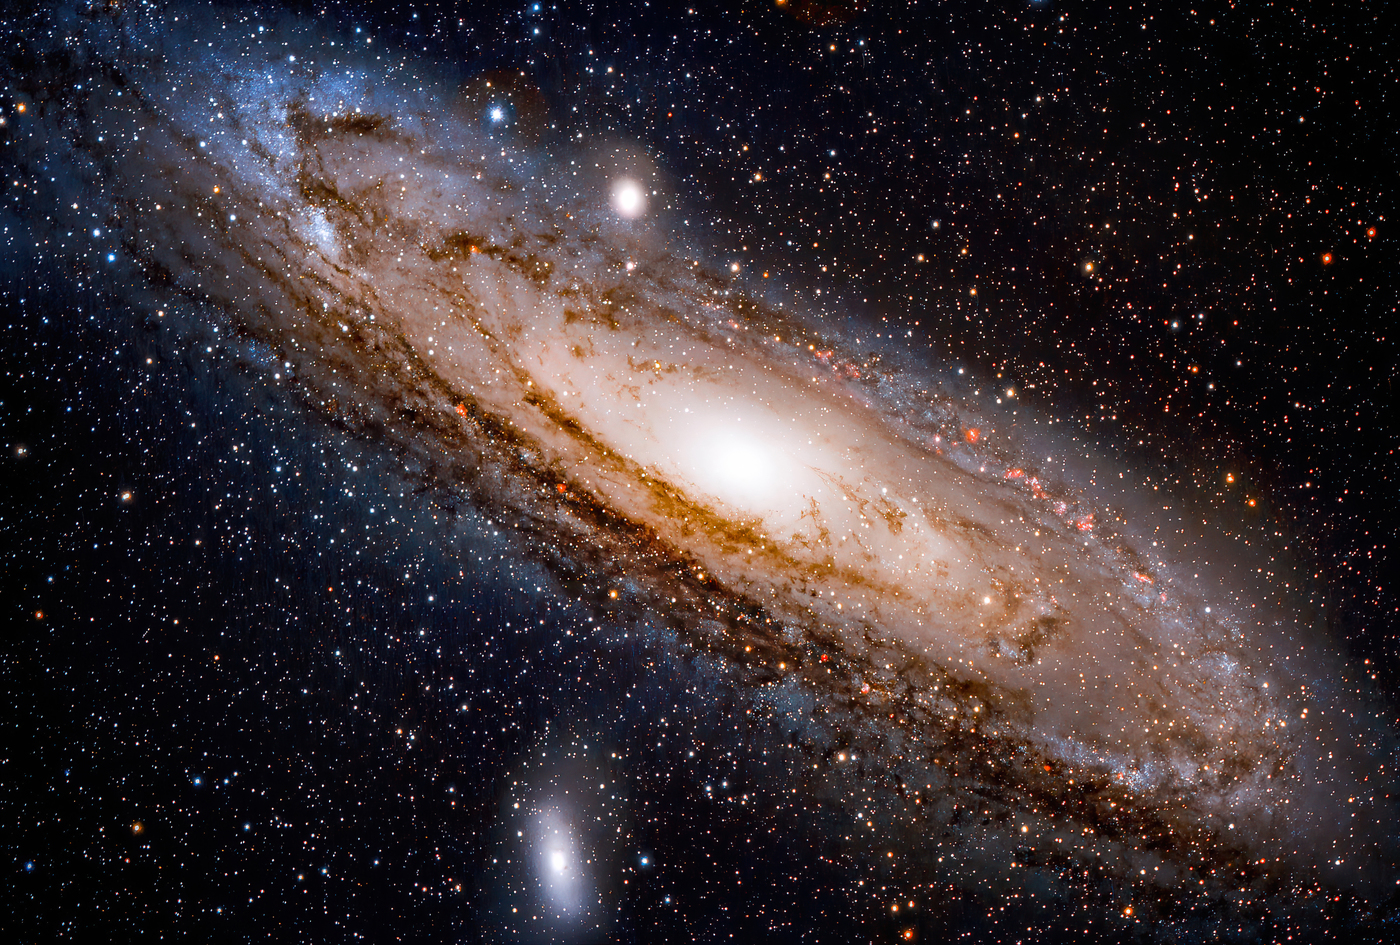
\includegraphics[width=0.99\columnwidth]{images/M31.jpg}\caption{Галактика Туманность Андромеды (М31)}\end{figure}}
\vs p012 2:3 В недалёком будущем новые телескопы\fnst{Согласно книге \cite{Baker1} здесь, видимо, речь идёт о 200\hyp{}дюймовом телескопе Hale, спонсированном Фондом Рокфеллера в 1928 году. Его строительство началось в 1936 году и завершилось в 1948 году.} откроют удивлённому взору астрономов Урантии не менее 375\,000\,000 новых\fnst{По книге \cite{Baker1} новый 200\hyp{}дюймовый телескоп откроет взору <<более чем 200 миллионов галактик>>.} галактик в отдалённых областях внешнего пространства. В то же время эти более мощные телескопы покажут, что многие островные вселенные\fnst{Так раньше назывались галактики (англ. island universes). Этот термин используется сэром Джеймсом Джинсом (книги которого являются ключевыми источниками текста Пятого Эпохального Откровения), хотя введён он был значительно раньше английским астрономом Уильямом Гершелем.}, ранее считавшиеся находящимися во внешнем пространстве, на самом деле являются частью галактической системы Орвонтон. Семь сверхвселенных всё ещё растут; периферия каждой из них постепенно расширяется; новые туманности постоянно стабилизируются и организуются; и некоторые из туманностей, которые астрономы Урантии считают внегалактическими, на самом деле находятся на окраине Орвонтона и путешествуют вместе с нами\fnst{Возможно, что речь идёт о Большом и Малом Магеллановых Облаках.}.\tunemarkup{pictures}{\begin{figure}[H]\centering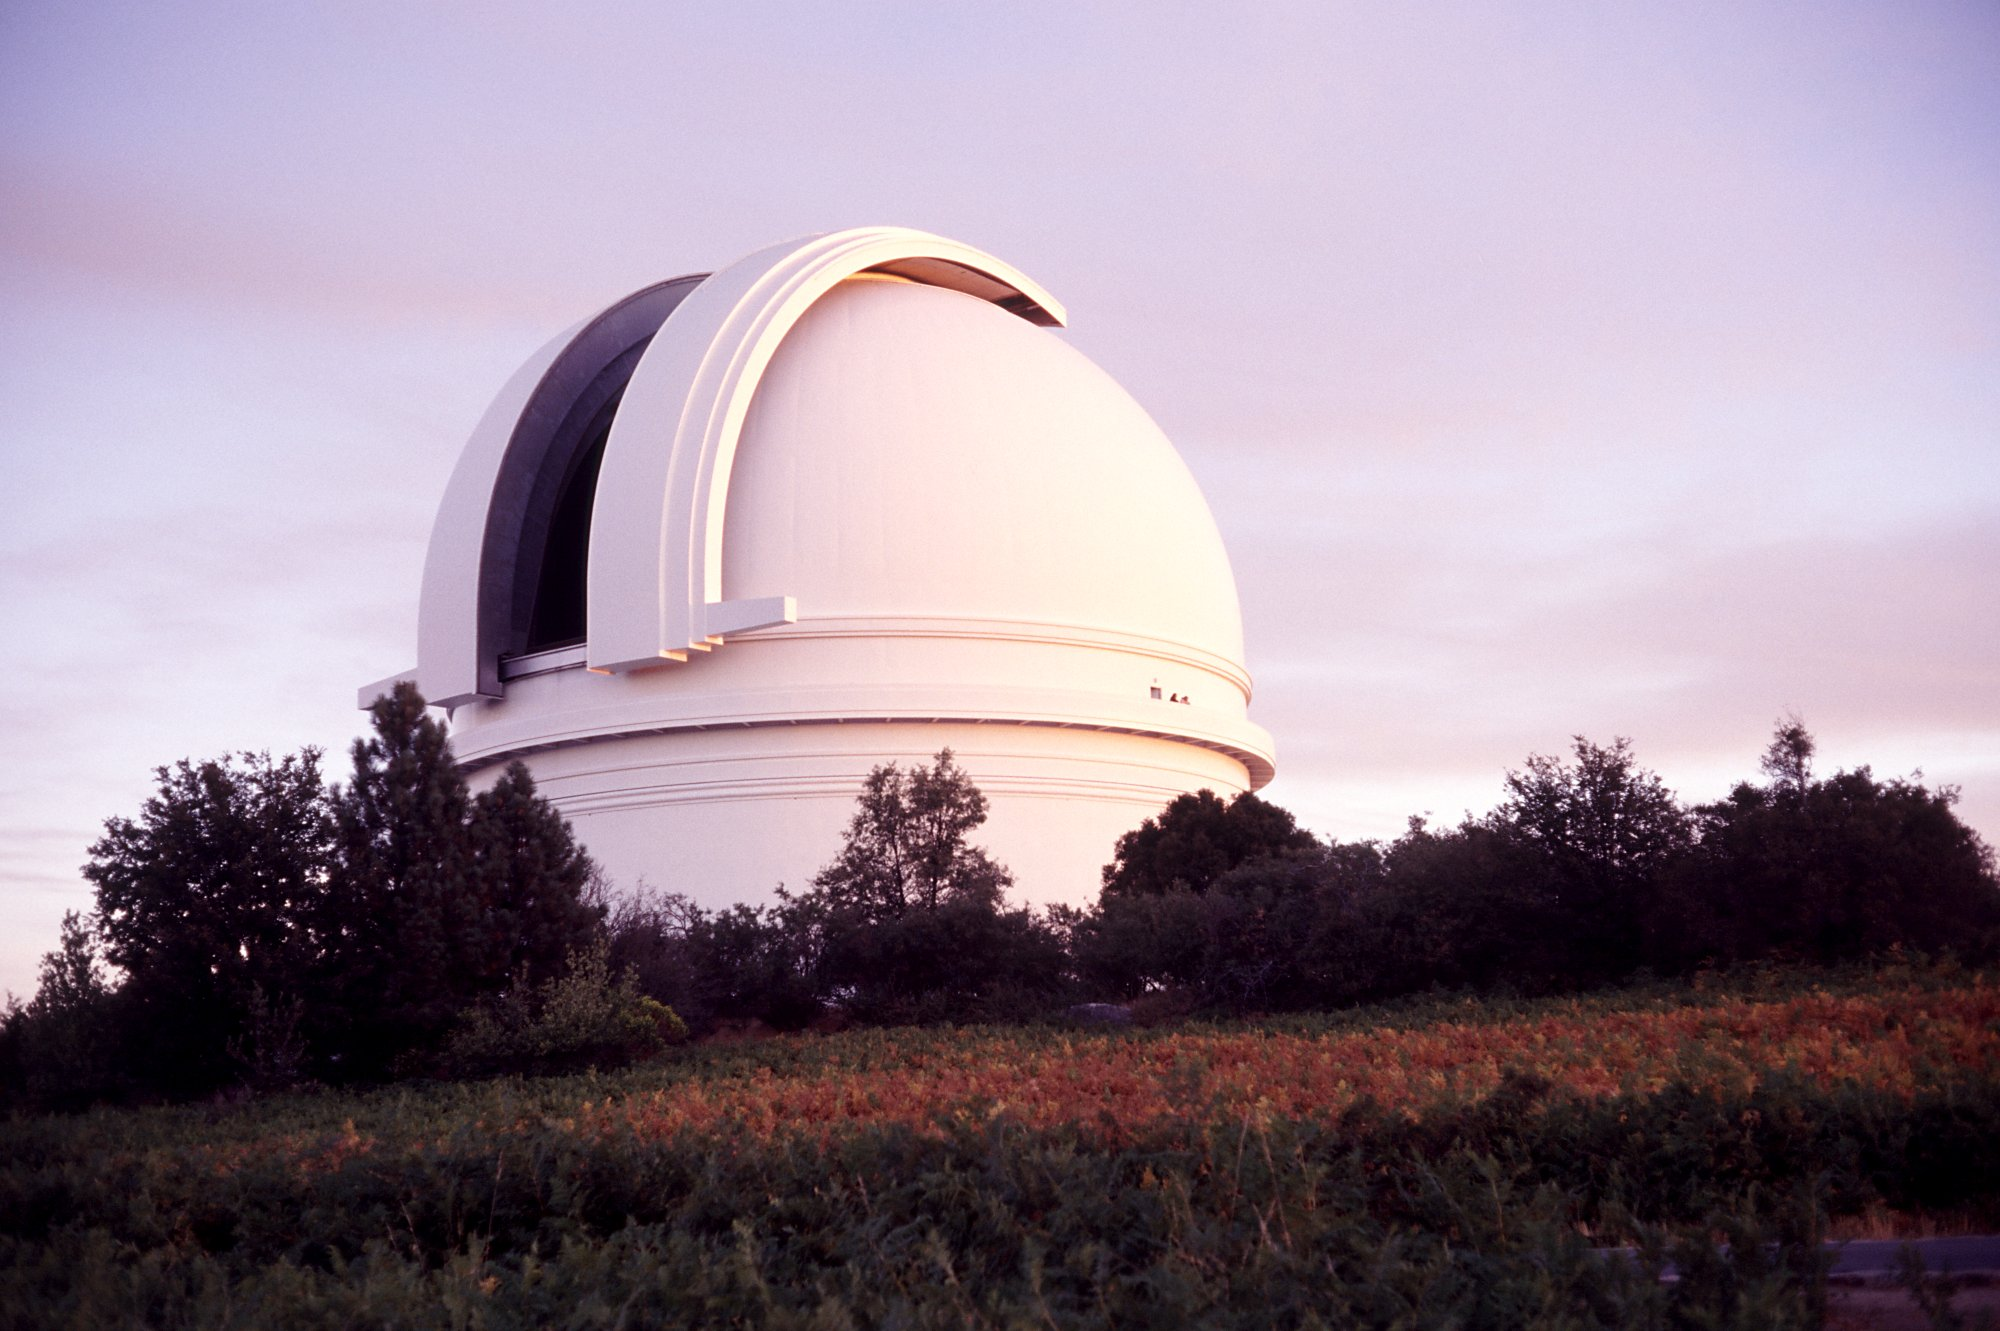
\includegraphics[width=0.92\columnwidth]{images/Hale-200inch.jpg}\caption{200\hyp{}дюймовый телескоп George Ellery Hale Паломарской обсерватории в Сан\hyp{}Диего, Калифорния, США}\end{figure}}
\vs p012 2:4 \pc Астрономы [star students] Уверсы отмечают, что большая вселенная окружена предшественниками ряда звёздных и планетарных скоплений, которые полностью окружают нынешнее обитаемое творение в виде концентрических колец внешних многочисленных вселенных. Физики Уверсы подсчитали, что энергия и материя этих внешних и неизведанных областей уже во много раз превышают общую материальную массу и энергетический заряд, заключённый во всех семи сверхвселенных. Мы знаем, что превращение космической силы в этих внешних пространственных уровнях является функцией Райских организаторов силы. Мы также знаем, что эти силы предшествуют тем физическим энергиям, которые в настоящее время активируют большую вселенную. Однако управляющие энергией Орвонтона не имеют никакого отношения к этим удалённым мирам, а движения энергии в них не связаны явным образом с контурами мощи организованных и обитаемых творений.\tunemarkup{pictures}{\begin{figure}[H]\centering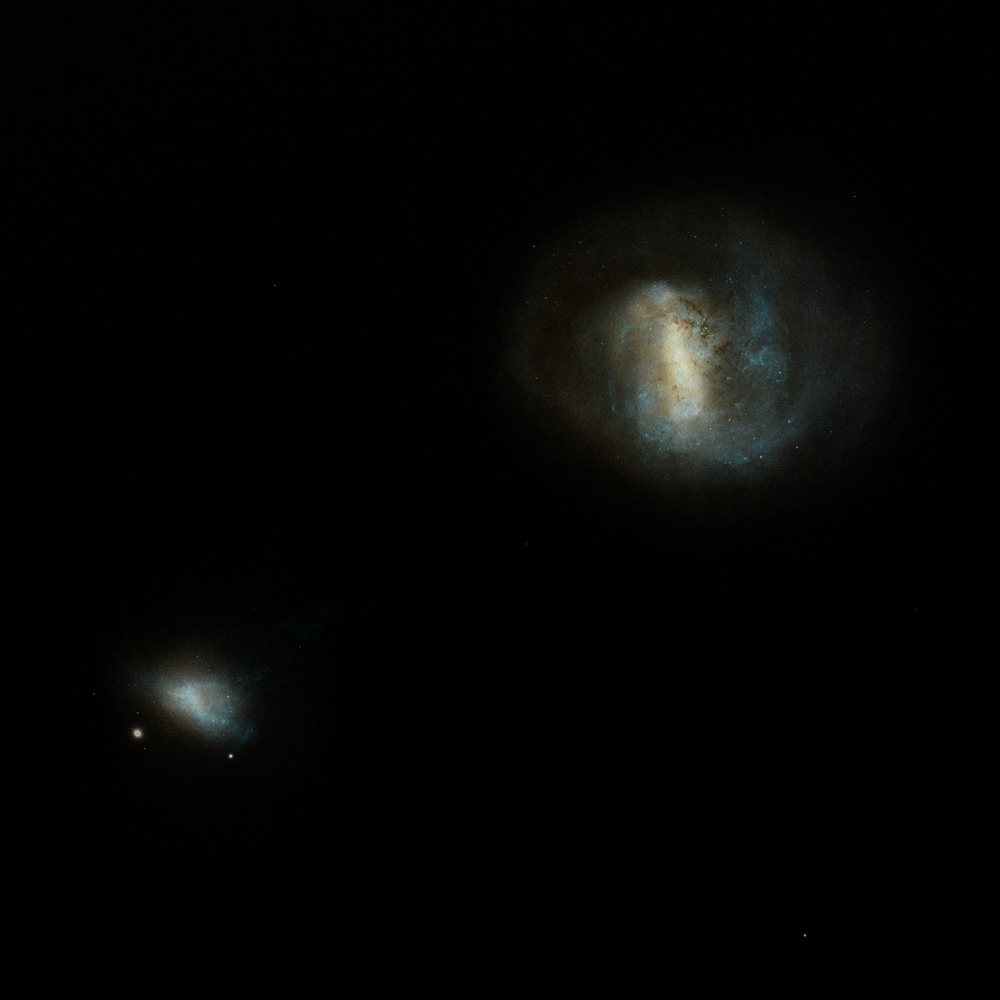
\includegraphics[width=0.9\columnwidth]{images/LMC.jpg}\caption{Большое и Малое Магеллановы Облака}\end{figure}}
\vs p012 2:5 \pc Мы очень мало знаем о значении этих грандиозных явлений внешнего пространства. Ещё более великое творение будущего находится в процессе формирования. Мы наблюдаем его необъятность, мы можем различать его протяжённость и ощущать его величественные размеры, но в остальном мы знаем об этих сферах немногим больше, чем астрономы Урантии. Насколько нам известно, в этом внешнем кольце туманностей, солнц и планет нет материальных существ вроде людей, ангелов или других духовных созданий. Эта далёкая область находится вне юрисдикции и управления правительств сверхвселенных.
\vs p012 2:6 По всему Орвонтону бытует мнение, что имеет место процесс творения нового типа вселенных, которым суждено стать ареной будущих действий собирающегося Корпуса Завершения; и если наши предположения верны, то бесконечное будущее может принести всем вам те же захватывающие дух зрелища, которые бесконечное прошлое содержало для ваших старших поколений [seniors] и предшественников.
\usection{ВСЕОБЩАЯ ГРАВИТАЦИЯ}
\vs p012 3:1 Все формы силы\hyp{}энергии~--- материальной, ментальной или духовной~--- одинаково подвержены тому охвату, тем универсальным присутствиям, которые мы называем гравитацией. Личность также восприимчива к гравитации~--- исключительному контуру Отца; но, хотя этот контур специфически относится именно к Отцу, он\fnst{Отец, а не контур.} не исключён из других контуров; Всеобщий Отец бесконечен и действует по \bibemph{всем} четырём контурам абсолютной гравитации в главной вселенной:
\vs p012 3:2 \li{1.}Гравитация личности Всеобщего Отца.
\vs p012 3:3 \li{2.}Гравитация духа Вечного Сына.
\vs p012 3:4 \li{3.}Гравитация разума Совместного Вершителя.
\vs p012 3:5 \li{4.}Космическая гравитация Острова Рай.
\vs p012 3:6 \pc Эти четыре контура не имеют отношения к силовому центру нижнего Рая; они не являются ни силовыми, ни энергетическими, ни мощностными контурами. Они представляют собой контуры абсолютного \bibemph{присутствия} и, подобно Богу, не зависят от времени и пространства.
\vs p012 3:7 В этой связи интересно упомянуть результаты некоторых наблюдений, сделанных на Уверсе в течение последних тысячелетий корпусом исследователей гравитации. Эта группа экспертов пришла к следующим выводам относительно различных гравитационных систем главной вселенной:
\vs p012 3:8 \li{1.}\bibemph{Физическая гравитация}. Оценив результат суммирования полного потенциала физической гравитации большой вселенной, они тщательно сравнили его с оценкой полной величины ныне действующего присутствия абсолютной гравитации. Эти расчёты показывают, что общее гравитационное воздействие на большую вселенную составляет очень малую часть предполагаемого гравитационного притяжения Рая, вычисленного на основе реакции элементарных физических единиц вселенской материи на гравитацию. Эти исследователи приходят к удивительному выводу, что центральная вселенная и окружающие её семь сверхвселенных в настоящее время используют только около 5\% активно функционирующего охвата абсолютной гравитации Рая. Иными словами: в настоящий момент около 95\% активного действия космической гравитации Острова Рай, вычисленного по этой теории тотальности, задействовано в управлении материальными системами за пределами существующих сегодня организованных вселенных. Все эти расчёты относятся к абсолютной гравитации; линейная гравитация~--- это явление взаимодействия, и её можно вычислить, только зная фактическую величину гравитации Рая.
\vs p012 3:9 \li{2.}\bibemph{Духовная гравитация}. Тем же самым методом сравнительной оценки и расчёта эти исследователи изучили текущую способность отклика гравитации духа и, в сотрудничестве с Одинокими Посланниками и другими духовными личностями, получили суммарную величину активной гравитации духа Второго Источника и Центра. И, что особенно поучительно, они обнаружили примерно такое же значение для фактического и функционального присутствия гравитации духа в большой вселенной, какое постулируется ими для полной суммы активной гравитации духа в настоящее время. Иными словами: в настоящее время практически вся гравитация духа Вечного Сына, вычисленная по этой теории тотальности, наблюдается функционирующей в большой вселенной. Если эти открытия достоверны, мы можем заключить, что вселенные, которые сейчас развиваются во внешнем пространстве, в настоящее время полностью недуховны. И если это так, это удовлетворительно объясняет, почему наделённые духом существа почти ничего не знают об этих громадных проявлениях энергии, кроме самог\'о факта их физического существования.
\vs p012 3:10 \li{3.}\bibemph{Гравитация разума}. Используя те же принципы сравнительных вычислений, эти специалисты приступили к решению задачи о присутствии гравитации разума и реакции на неё. Единица разума, принятая для оценки, была получена усреднением трёх материальных и трёх духовных складов ума, хотя тип разума, присутствующий в управляющих мощью и их партнёрах, оказался мешающим фактором при определении базовой единицы для оценки гравитации разума. В соответствии с данной теорией тотальности оказалось несложным оценить нынешнюю способность Третьего Источника и Центра для функции гравитации разума. Хотя результаты в данном случае не столь убедительны, как в оценках физической и духовной гравитации, при сравнительном рассмотрении они весьма поучительны и даже загадочны. Эти исследователи пришли к выводу, что около 85\% реакции гравитации разума на интеллектуальное притяжение Совместного Вершителя берёт начало в существующей большой вселенной. Это указывает на возможность того, что наблюдаемые физические процессы, ныне происходящие по всем областям внешнего пространства, связаны с активностью разума\fnst{А именно: с остальными 15\% от общей активности разума.}. Хотя эта оценка, вероятно, далеко не точна, она в принципе согласуется с нашими представлениями о том, что разумные организаторы сил в настоящее время направляют эволюцию вселенной на пространственных уровнях за пределами нынешних внешних границ большой вселенной. Какой бы ни была природа этого постулируемого разума, очевидно, что он не реагирует на гравитацию духа.
\vs p012 3:11 Но все эти вычисления в лучшем случае являются оценками, основанными на предполагаемых законах. Мы думаем, что они достаточно надёжны. Даже если несколько духовных существ находятся во внешнем пространстве, их коллективное присутствие не может заметным образом повлиять на вычисления, касающиеся таких масштабных измерений.
\vs p012 3:12 \pc \bibemph{Гравитация личности} невычислима. Мы распознаём этот контур, но не можем измерить ни качественные, ни количественные реальности, реагирующие на него.
\usection{ПРОСТРАНСТВО И ДВИЖЕНИЕ}
\vs p012 4:1 Все единицы космической энергии находятся в первичном вращении, заняты выполнением своей миссии, обращаясь по вселенской орбите. Вселенные пространства и их составные системы и миры представляют собой вращающиеся сферы, движущиеся по бесконечным контурам уровней пространства главной вселенной. Во всей главной вселенной нет абсолютно ничего неподвижного, кроме с\'амого центра Хавоны, вечного Острова Рай, центра гравитации.
\vs p012 4:2 Безусловный Абсолют функционально ограничен пространством, но мы не столь уверены относительно связи этого Абсолюта с движением. Присуще ли ему движение? Мы не знаем. Мы знаем, что движение не присуще пространству; даже движения \bibemph{самог\'о} пространства не являются врождёнными. Но мы не столь уверены относительно связи Безусловного с движением. Кто или что на самом деле отвечает за гигантские процессы трансмутации силы\hyp{}энергии, которые сейчас продолжаются за пределами нынешних семи сверхвселенных? Относительно происхождения движения у нас есть следующие мнения:
\vs p012 4:3 \li{1.}Мы думаем, что Совместный Вершитель инициирует движение \bibemph{в} пространстве.
\vs p012 4:4 \li{2.}Если Совместный Вершитель и производит движения \bibemph{самог\'о} пространства, мы не можем этого доказать.
\vs p012 4:5 \li{3.}Всеобщий Абсолют не порождает первоначальное движение, но он стабилизирует и контролирует все напряжения, порождаемые движением.
\vs p012 4:6 \pc Во внешнем пространстве организаторы сил, по\hyp{}видимому, отвечают за создание гигантских вселенских дисков, которые сейчас находятся в процессе звёздообразования, но их способность функционировать таким образом, должно быть, стала возможной благодаря некоторой модификации космического присутствия Безусловного Абсолюта.\tunemarkup{pictures}{\begin{figure}[H]\centering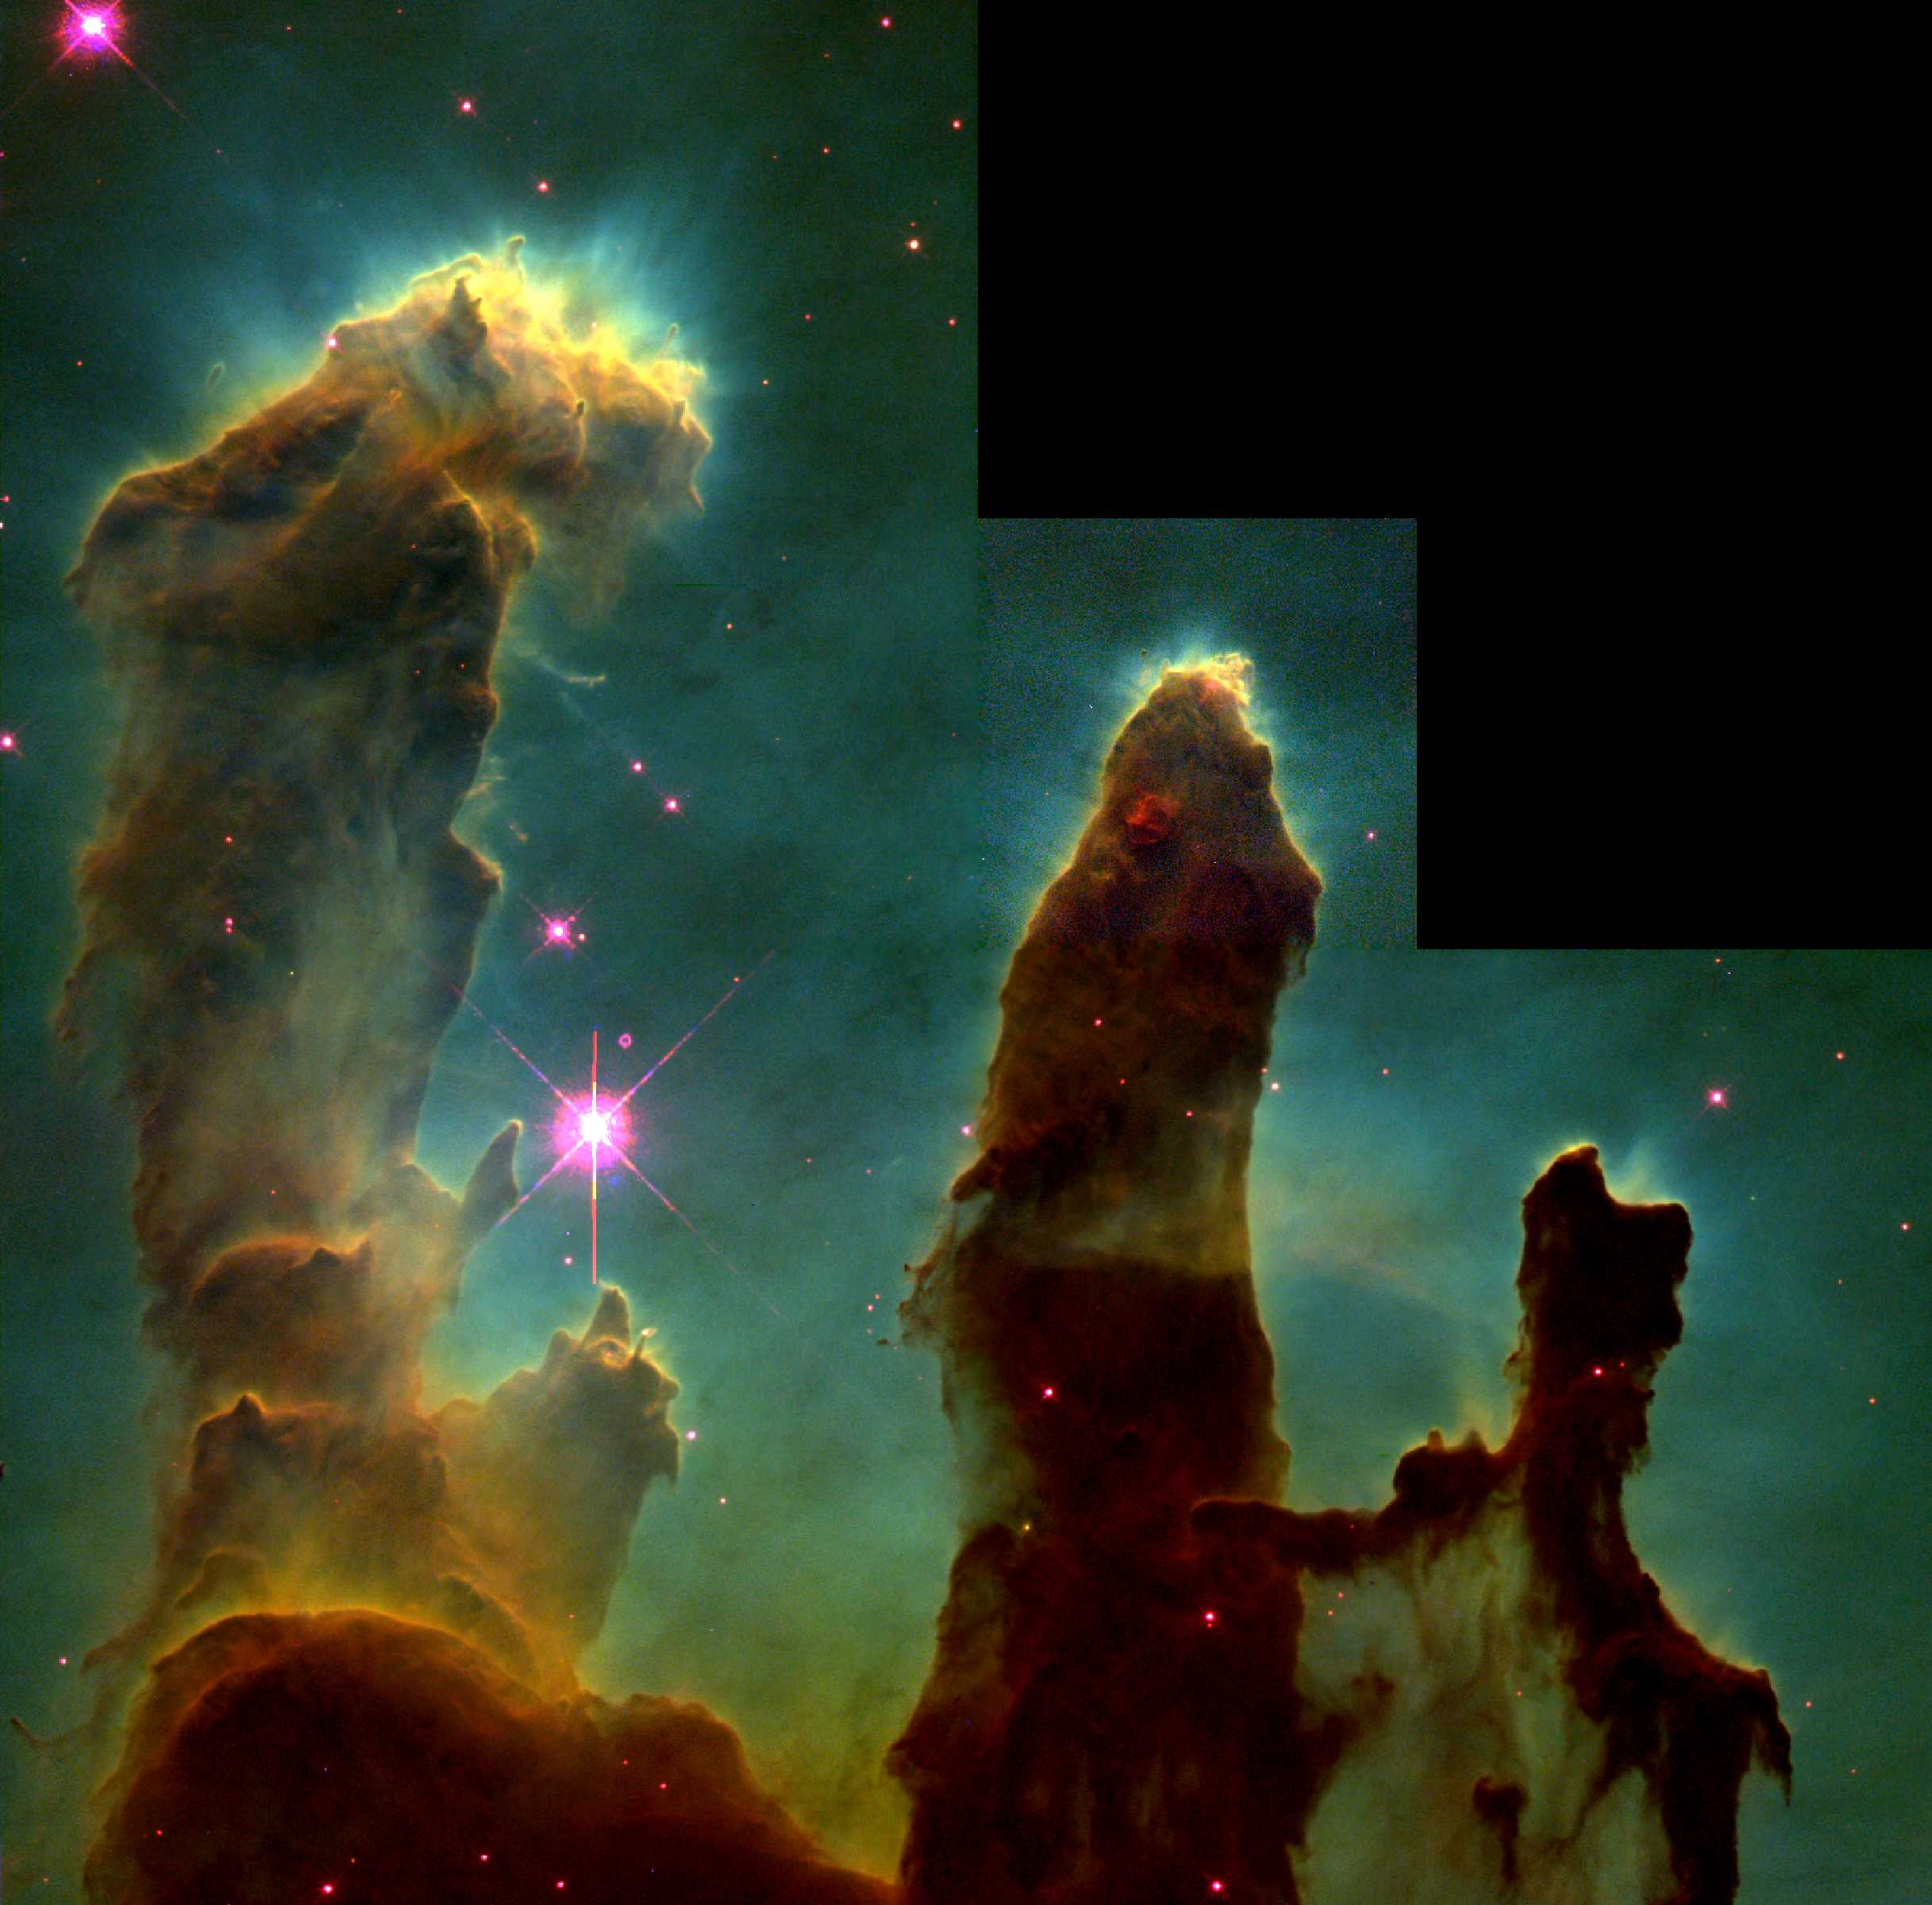
\includegraphics[width=0.99\columnwidth]{images/Stolpy-tvoreniya.jpg}\caption{<<Столпы творения>> в туманности Орёл}\end{figure}}
\vs p012 4:7 \pc Пространство, с человеческой точки зрения,~--- это ничто, нечто отрицательное; оно существует только по отношению к чему\hyp{}то положительному и непространственному. Тем не менее пространство реально. Оно содержит и обуславливает движение. Оно даже движется. Движения пространства можно приблизительно классифицировать следующим образом:
\vs p012 4:8 \li{1.}Первичное движение~--- респирация\fnst{Дыхание.} пространства, движение самог\'о пространства.
\vs p012 4:9 \li{2.}Вторичное движение~--- противоположно направленные обращения последовательных уровней пространства.
\vs p012 4:10 \li{3.}Относительные движения~--- относительные в том смысле, что они не вычисляются относительно Рая как точки отсчёта. Первичные и вторичные движения абсолютны, это движения относительно неподвижного Рая.
\vs p012 4:11 \li{4.}Компенсирующее или коррелирующее перемещение, предназначенное для координации всех остальных типов движения.
\vs p012 4:12 \pc Нынешнее взаимоотношение вашего Солнца и связанных с ним планет хотя и раскрывает множество относительных и абсолютных движений в пространстве, но создаёт впечатление у астрономов\hyp{}наблюдателей, что вы сравнительно неподвижны в пространстве, а ваши вычисления, охватывающие всё новые глубины пространства, указывают на то, что окружающие звёздные скопления и потоки вовлечены в направленный вовне полёт с постоянно возрастающими скоростями. Но это не так. Вы не принимаете во внимание нынешнее однородное расширение физических творений всего насыщенного пространства. Ваше собственное локальное творение (Небадон) участвует в этом движении всеобщего расширения. Все семь сверхвселенных участвуют в цикле пространственной респирации, длительностью в два миллиарда лет, вместе с внешними областями главной вселенной.
\vs p012 4:13 Когда вселенные расширяются и сжимаются, материальные массы в насыщенном пространстве попеременно движутся против и по направлению притяжения Райской гравитации. Работа, совершаемая при перемещении материальной энергетической массы творения, есть работа \bibemph{пространственная,} а не работа \bibemph{мощи\hyp{}энергии}.
\vs p012 4:14 \pc Хотя ваши спектроскопические оценки астрономических скоростей достаточно надёжны в применении к звёздным мирам, принадлежащим вашей и соседним сверхвселенным, такие расчёты совершенно непригодны к мирам внешнего пространства. Спектральные линии приближающейся звезды смещены в фиолетовую сторону; и, наоборот, у удаляющейся звезды эти линии смещаются в красную сторону. Многие факторы, накладываясь, создают впечатление, будто скорость удаления внешних вселенных увеличивается с расстоянием более чем на 160~км/с на каждый 1\,000\,000 световых лет\fnst{Приведённое в тексте Откровения значение постоянной Хаббла (522\,км/c/Мпк) близко к полученному самим Хабблом в 1935\,г. значению 535\,км/с/Мпк. Вычисления Хаббла были основаны на зависимости между периодом и светимостью переменных звёзд, именуемых цефеидами. Пересмотр нуль\hyp{}пункта этой зависимости (В.\,Бааде, 1952\,г.) привёл к коррекции величины постоянной Хаббла. К 1955\,г. общепринятым значением являлось 180\,км/с/Мпк. Современное (2016\,г.) значение и того меньше: 66,93$\pm$0,62\,км/с/Мпк.}. С усовершенствованием более мощных телескопов подобные рассуждения приведут к выводу, что эти далёкие системы удаляются из данной части вселенной с невероятной скоростью, превышающей 48\,000~км/с. Но эта кажущаяся скорость удаления нереальна; она является результатом множества факторов, приводящих к ошибке, включая углы наблюдения и другие время\hyp{}пространственные искажения\fnst{На эту возможность указал в 1920 году Эддингтон в своей книге <<Пространство, время и тяготение>>. См. главу~XI в \cite{Eddington1} (имеется перевод книги на русский язык \cite{Eddington2}).}.
\vs p012 4:15 Но наибольшее искажение возникает из\hyp{}за того, что огромные вселенные внешнего пространства в сферах, следующих за областями семи сверхвселенных, по\hyp{}видимому, вращаются в направлении, противоположном направлению вращения большой вселенной. То есть эти мириады туманностей и сопровождающих их солнц и сфер в настоящее время вращаются по часовой стрелке вокруг центрального творения. Семь сверхвселенных вращаются вокруг Рая против часовой стрелки. Представляется, что вторая внешняя вселенная галактик, как и семь сверхвселенных, вращается против часовой стрелки вокруг Рая. И астрономы\hyp{}наблюдатели Уверсы полагают, что они обнаружили доказательства вращательных движений в третьем внешнем поясе далёкого пространства, которые начинают проявлять тенденции направленности по часовой стрелке.
\vs p012 4:16 Вероятно, что эти попеременные направления последовательных процессий вселенных в пространстве имеют какое\hyp{}то отношение к механизму гравитации Всеобщего Абсолюта, действующему внутри главной вселенной и заключающемуся в координации сил и выравнивании пространственных напряжений. Движение, так же как и пространство, дополняет или уравновешивает гравитацию.
\usection{ПРОСТРАНСТВО И ВРЕМЯ}
\vs p012 5:1 Как и пространство, время есть дар Рая, но не в том же смысле, а лишь косвенно. Время возникает благодаря движению и потому, что разум изначально осознаёт последовательность. С практической точки зрения движение является существенным для времени, однако не существует универсальной единицы времени, основанной на движении, за исключением стандартного дня Рая\hyp{}Хавоны, произвольно принятого за таковую. Тотальность респирации пространства разрушает его локальную ценность в качестве источника времени.
\vs p012 5:2 Пространство не бесконечно, хотя оно и берёт начало из Рая; не абсолютно, ибо оно пронизано Безусловным Абсолютом. Мы не знаем абсолютных пределов пространства, но мы знаем, что абсолютом времени является вечность.
\vs p012 5:3 \pc Время и пространство неразделимы только во время\hyp{}пространственных творениях~--- семи сверхвселенных. Нетемпоральное пространство (пространство без времени) теоретически существует, но единственным действительно нетемпоральным местом является \bibemph{площадь}\fnst{Именно \bibemph{площадь} (англ. \bibemph{area}). Связано ли это как\hyp{}то со свойством фазового пространства, в котором не существует расстояния между двумя точками $(x_1,p_1)$ и $(x_2,p_2)$, но вполне можно говорить о \bibemph{площади} треугольника с вершинами в трёх точках $(x_1,p_1)$, $(x_2,p_2)$ и $(x_3,p_3)$? Именно эта площадь странным образом фигурирует в эволюционных пропагаторах квантовой механики, переформулированной в терминах функций Вигнера.} Рая. Непространственное время (время без пространства) существует в разуме, функционирующем на уровне Рая.
\vs p012 5:4 Относительно неподвижные зоны промежуточного пространства, примыкающие к Раю и отделяющие насыщенное пространство от ненасыщенного, являются зонами перехода от времени к вечности, поэтому Райские пилигримы должны терять сознание во время этого перехода, когда он должен увенчаться Райским гражданством. Сознающие время \bibemph{посетители} могут попасть в Рай, не впадая в такой сон, но они остаются созданиями времени.
\vs p012 5:5 \pc Временн\'ые связи не существуют без движения в пространстве, но осознание времени существует. Понятие последовательности\fnst{Видимо, <<последовательности событий>>.} позволяет осознавать время даже в отсутствие движения. По своей природе человеческий разум меньше привязан ко времени, чем к пространству. Даже во дни земной жизни во плоти человеческий разум жёстко привязан к пространству, в то время как творческое воображение человека относительно свободно от времени. Но само время не является генетическим качеством разума.
\vs p012 5:6 \pc Существует три разных уровня восприятия времени\fnst{В то время как существует \bibemph{семь} различных концепций пространства, обусловленного временем. См.\,\bibref[130:7.6]{p130 7:6}.}:
\vs p012 5:7 \li{1.}Время, воспринимаемое разумом,~--- осознание последовательности, движения и ощущение продолжительности.
\vs p012 5:8 \li{2.}Время, воспринимаемое духом,~--- проникновение в суть движения по направлению к Богу и осознание восходящего движения по уровням возрастающей божественности.
\vs p012 5:9 \li{3.}Личность \bibemph{создаёт} уникальное чувство времени из проникновения в суть Реальности плюс сознания присутствия и осознания продолжительности.
\vs p012 5:10 \pc Бездуховные животные знают только прошлое и живут настоящим. Человек, в котором пребывает дух, обладает способностью предвидения (проницательности); он может представить себе будущее. Только обращённые в будущее и прогрессивные взгляды являются реальными для личности. Статическая этика и традиционная мораль лишь немного сверхживотны. Не является высоким видом самореализации и стоицизм. Этика и мораль становятся истинно человеческими тогда, когда они динамичны и прогрессивны, наполнены жизнью вселенской реальности.
\vs p012 5:11 Человеческая личность не просто сопутствует время\hyp{}пространственным событиям; человеческая личность может также действовать в качестве космической причины таких событий\fnst{Эта мысль взята из замечательной книги H.A.~Overstreet, <<The Enduring Quest: A Search for a Philosophy of Life>> \cite{Overstreet1}.}.
\usection{ВСЕОБЩЕЕ СВЕРХУПРАВЛЕНИЕ}
\vs p012 6:1 Вселенная не статична. Стабильность~--- не результат инерции, но, скорее, результат сбалансированных энергий, сотрудничающих разумов, скоординированных моронтий, сверхконтроля духа и объединения личности. Стабильность целиком и всегда пропорциональна божественности.
\vs p012 6:2 В физическом управлении главной вселенной Всеобщий Отец осуществляет приоритет и первенство через Остров Рай; Бог абсолютен в духовном управлении космосом в лице Вечного Сына. Что касается областей разума, Отец и Сын согласованно действуют в Совместном Вершителе.
\vs p012 6:3 Третий Источник и Центр помогает в поддержании равновесия и координации объединённых физических и духовных энергий и формирований посредством абсолютности своего охвата космического разума и благодаря проявлению присущих ему и универсальных дополнений физической и духовной гравитации. Когда бы и где бы ни возникала связь между материальным и духовным, такое явление разума является действием Бесконечного Духа. Только разум может осуществлять взаимосвязь физических сил и энергий материального уровня с духовными силами и существами уровня духа.
\vs p012 6:4 Во всех твоих размышлениях о вселенских явлениях убедись, что ты принимаешь во внимание взаимосвязь физических, интеллектуальных и духовных энергий и что должным образом учитываешь неожиданные явления, сопровождающие их объединение личностью, и непредсказуемые явления, возникающие в результате действия и реакции эмпирического Божества и Абсолютов.
\vs p012 6:5 Вселенная в высшей степени предсказуема только в количественном смысле,~--- в смысле измерения гравитации; даже первичные физические силы не реагируют на линейную гравитацию, равно как и смыслы высшего разума и истинные духовные ценности предельных вселенских реальностей. В качественном смысле Вселенная не очень предсказуема в отношении новых ассоциаций сил~--- физических, ментальных или духовных,~--- хотя многие такие комбинации энергий или сил становятся частично предсказуемыми, когда подвергаются критическому наблюдению. Когда материя, разум и дух объединены личностью создания, мы не можем полностью предсказать решения такого существа, обладающего свободной волей.
\vs p012 6:6 \pc Все фазы изначальной силы, зарождающегося духа и других неличностных предельностей, по\hyp{}видимому, реагируют в соответствии с некоторыми относительно стабильными, но неизвестными законами и характеризуются широтой действия и гибкостью реакции, которые часто приводят в замешательство, когда встречаются в явлениях ограниченных и изолированных ситуаций. Каково объяснение этой непредсказуемой свободы реакции, обнаруживаемой этими возникающими вселенскими актуальностями? Эти неизвестные, непостижимые непредсказуемости,~--- относятся ли они к поведению первичной единицы силы, реакции неопознанного уровня разума или феномену обширной предвселенной, создаваемой в областях внешнего пространства,~--- вероятно, раскрывают деятельность Предельного и присутствие\hyp{}действие Абсолютов, предшествующих функционированию всех вселенских Создателей.
\vs p012 6:7 Хотя доподлинно нам это неизвестно, мы предполагаем, что такая удивительная разносторонность и такая глубокая координация означают присутствие и действие Абсолютов, и что такое разнообразие реакций при явно однородной причинности раскрывает реакцию Абсолютов,~--- и не только на непосредственную и ситуативную причину, но также и на все другие родственные причины по всей главной вселенной.
\vs p012 6:8 \pc У индивидуумов есть свои хранители предназначения; планеты, системы, созвездия, вселенные и сверхвселенные~--- все имеют своих соответствующих правителей, которые трудятся на благо своих владений. За Хавоной, и даже большой вселенной, наблюдают те, кому доверена столь высокая ответственность. Но кто взращивает и заботится о фундаментальных потребностях главной вселенной в целом~--- от Рая до четвёртого и самого дальнего пространственного уровня? Экзистенциально такую сверхзаботу, вероятно, можно приписывать Райской Троице, но с эмпирической точки зрения появление вселенных после Хавоны зависит от:
\vs p012 6:9 \li{1.}Абсолютов~--- в потенциале.
\vs p012 6:10 \li{2.}Предельного~--- в направлении.
\vs p012 6:11 \li{3.}Верховного~--- в эволюционной координации.
\vs p012 6:12 \li{4.}Зодчих Главной Вселенной~--- в управлении до появления специальных правителей.
\vs p012 6:13 \pc Безусловный Абсолют пронизывает всё пространство. Нам не вполне ясен точный статус Божественного и Всеобщего Абсолютов, но мы знаем, что последний действует везде, где действуют Божественный и Безусловный Абсолюты. Божественный Абсолют может присутствовать повсюду, но вряд ли возможно его пространственное присутствие. Предельный присутствует или когда\hyp{}нибудь будет присутствовать в пространстве до внешних границ четвёртого пространственного уровня. Мы сомневаемся, что Предельный будет когда\hyp{}либо иметь пространственное присутствие за периферией главной вселенной, но в этих границах Предельный постепенно объединяет творческую структуру потенциалов трёх Абсолютов.
\usection{ЧАСТЬ И ЦЕЛОЕ}
\vs p012 7:1 Во всём времени и пространстве и по отношению ко всей реальности любой природы действует неумолимый и беспристрастный закон, эквивалентный функции космического провидения. Милосердие характеризует отношение любви Бога к индивидууму; беспристрастность мотивирует отношение Бога к целому. Воля Бога не обязательно преобладает в части~--- в сердце любой отдельно взятой личности,~--- но его воля действительно управляет целым~--- вселенной вселенных.
\vs p012 7:2 \pc Истинно, что во всех его отношениях со всеми своими существами законы Бога не являются по своей сути произвольными. Тебе, с твоим ограниченным в\'идением и конечной точкой зрения, деяния Бога часто должны казаться диктаторскими и произвольными. Законы Бога~--- это просто привычки Бога\fnst{Эта мысль взята из книги J.~Strong, <<The New World\hyp{}Religion>> \cite{Strong1}.}, его способ делать что\hyp{}то повторяющееся; и он всегда всё делает хорошо. Ты можешь заметить, что Бог делает одно и то же тем же самым образом просто потому, что это лучший способ сделать эту конкретную вещь в данных обстоятельствах; а лучший способ и есть правильный, и поэтому бесконечная мудрость всегда предписывает, чтобы это было сделано именно таким точным и совершенным образом. Тебе следует также помнить, что природа не является исключительным действием Божества; другие влияния присутствуют в тех явлениях, которые человек называет природой.
\vs p012 7:3 Божественной природе невыносимо терпеть любую форму деградации или даже разрешать совершение какого\hyp{}либо чисто личного действия не самым лучшим образом. Однако следует прояснить, что \bibemph{если} в божественности любой ситуации, в экстремальности любых обстоятельств, в любом случае, когда следование верховной мудрости может указать требование иного поведения,~--- если требования совершенства по какой\hyp{}либо причине диктуют другой, лучший способ реагирования,~--- тогда премудрый Бог сразу же поступит таким лучшим и более подходящим способом. И это будет выражением высшего закона, а не отменой низшего.
\vs p012 7:4 Бог не является рабом привычки хронического повторения своих собственных добровольных действий. Между законами Бесконечного нет противоречий; все они~--- совершенства непогрешимой природы; все они~--- неоспоримые действия, выражающие безупречные решения. Закон~--- это неизменная реакция бесконечного, совершенного и божественного разума. Все деяния Бога являются волевыми, несмотря на их кажущуюся одинаковость. В Боге <<нет ни изменчивости, ни тени перемены>>\fnst{Цитата из Иакова~1:17.}. Но всё то, что может воистину быть сказано о Всеобщем Отце, не может быть с такой же уверенностью сказано обо всех подчинённых ему разумных существах или о его эволюционных созданиях.
\vs p012 7:5 Поскольку Бог неизменен, ты можешь во всех обычных обстоятельствах положиться на то, что он делает то же самое таким же идентичным и обычным образом. Бог~--- гарантия стабильности для всех созданных вещей и существ. Он Бог; поэтому он не меняется.
\vs p012 7:6 И всё это постоянство поведения и единообразие действий являются личными, сознательными и в высшей степени волевыми, ибо великий Бог не является беспомощным рабом своего собственного совершенства и бесконечности. Бог~--- это не самодействующая автоматическая сила; он не рабская законопослушная власть. Бог~--- это ни математическое уравнение, ни химическая формула. Он~--- первичная личность, обладающая свободой воли. Он является Всеобщим Отцом, существом, преисполненным личностью, и универсальным источником личности всех созданий.
\vs p012 7:7 \pc Воля Бога не постоянно побеждает в сердце ищущего Бога материального смертного, но если временн\'ые рамки расширить за пределы данного момента, охватывая всю первую жизнь, тогда воля Бога становится всё более заметной в духовных плодах, принесённых в жизнях ведомых духом детей Божьих. А затем, если человеческую жизнь ещё больше расширить, включив моронтийный опыт, то можно заметить, как божественная воля сияет всё ярче и ярче в одухотворяющих поступках тех созданий времени, которые начали ощущать вкус божественных наслаждений эмпирического переживания связи личности человека с личностью Всеобщего Отца.
\vs p012 7:8 Отцовство Бога и братство людей представляют собой парадокс части и целого на уровне личности. Бог любит \bibemph{каждого} индивидуума как отдельное дитя в небесной семье. В то же время Бог любит так же \bibemph{всех} индивидуумов; он нелицеприятен, и универсальность его любви порождает отношение целого~--- всеобщее братство.
\vs p012 7:9 Любовь Отца абсолютно индивидуализирует каждую личность как уникальное дитя Всеобщего Отца,~--- дитя без дубликатов в бесконечности, волевое создание, незаменимое во всей вечности. Любовь Отца возносит каждое дитя Бога, озаряя каждого члена небесной семьи, резко выделяя уникальную природу каждого личностного существа на фоне неличностных уровней, лежащих за пределами братского контура Отца всех. Любовь Бога поразительно отображает трансцендентную ценность каждого волевого создания, безошибочно раскрывает высокую ценность, которую Всеобщий Отец придаёт каждому из своих детей и всем им,~--- от высшей личности создателя с Райским статусом до низшей личности волевого достоинства среди диких племён на заре человеческого рода в каком\hyp{}нибудь эволюционном мире времени и пространства.
\vs p012 7:10 Именно эта любовь Бога к индивидууму порождает божественную семью всех индивидуумов, всеобщее братство добровольных детей Райского Отца. И это братство, будучи всеобщим, является отношением целого. Братство, если оно всеобщее, раскрывает не отношение \bibemph{каждого,} а отношение \bibemph{всех}. Братство~--- это реальность целого и поэтому раскрывает свойства целого в противоположность свойствам части.
\vs p012 7:11 Братство составляет факт отношения между каждой личностью во вселенском существовании. Ни одно лицо не может избежать преимуществ или потерь, которые могут возникнуть в результате отношений с другими лицами. Благополучие или страдания части соизмеримы с таковыми целого. Попытки каждого человека делать добро приносят пользу всем людям; ошибка или зло каждого человека усугубляет несчастье всех людей. Как движется часть, так движется и целое. Каков прогресс целого, таков прогресс и части. Относительные скорости части и целого определяют, будет ли часть замедляться инертностью целого или переноситься вперёд импульсом космического братства.
\vs p012 7:12 \pc Остаётся тайной, каким образом Бог, будучи высоколичностным, самосознающим существом, имеющим постоянную резиденцию, в то же самое время лично присутствует в такой огромной вселенной и лично находится в контакте практически с бесконечным числом существ. То, что данное явление является тайной за пределами человеческого понимания, не должно ни в коей мере умалять твою веру. Не позволяй громадности бесконечности, необъятности вечности, величию и славе несравненного характера Бога внушать тебе благоговейный страх, ошеломлять или обескураживать тебя; ибо Отец недалеко от любого из вас; он обитает внутри тебя, и в нём мы все буквально движемся, действительно живём и истинно обретаем наше бытие.
\vs p012 7:13 \pc Несмотря на то что Райский Отец действует через своих божественных создателей и своих детей\hyp{}созданий, он также поддерживает с тобой самую сокровенную связь,~--- связь столь возвышенную, столь высоко личную, что она выходит за пределы даже моего понимания,~--- то таинственное общение фрагмента Отца с человеческой душой и смертным разумом своего действительного пребывания. Исходя из того, что тебе уже известно об этих дарах Бога, ты должен понимать, что Отец находится в тесном контакте не только со своими божественными партнёрами, но и со своими эволюционными смертными детьми времени. Отец действительно обитает на Рае, но его божественное присутствие также обитает в разумах людей.
\vs p012 7:14 Хотя дух Сына и был излит на всю плоть, хотя Сын и жил когда\hyp{}то с вами в подобии смертной плоти, хотя серафимы лично охраняют и ведут вас, как может любое из этих божественных существ Второго и Третьего Центров надеяться подойти к вам так же близко или понять вас так же полно, как Отец, который отдал часть себя, чтобы быть в вас, чтобы быть вашим настоящим, божественным и даже вашим вечным <<я>>?
\usection{МАТЕРИЯ, РАЗУМ И ДУХ}
\vs p012 8:1 <<Бог есть дух>>, но Рай~--- нет. Материальная вселенная всегда является ареной, на которой происходит вся духовная деятельность; духовные существа и восходящие духи живут и работают на физических сферах материальной реальности.
\vs p012 8:2 \pc Дар космической силы, область космической гравитации~--- это функция Острова Рай. Вся изначальная сила\hyp{}энергия исходит из Рая, а материя для создания бессчётных вселенных в настоящее время циркулирует по всей главной вселенной в форме присутствия супергравитации, которое составляет силу\hyp{}заряд насыщенного пространства.
\vs p012 8:3 Какие бы трансформации ни претерпевала сила в далёких вселенных, выйдя из Рая, она продолжает путешествовать, подчиняясь нескончаемому, вездесущему, неизменному притяжению вечного Острова, послушно и присущим ей образом обращаясь по вечным пространственным траекториям вселенных. Физическая энергия~--- это единственная реальность, которая является верной и постоянной в своём подчинении всеобщему закону. Только в сферах воли созданий происходит отклонение от божественных путей и изначальных планов. Мощь и энергия~--- универсальные свидетельства стабильности, постоянства и вечности центрального Острова Рай.
\vs p012 8:4 \pc Посвящение духа и одухотворение личностей, сфера духовной гравитации~--- это сфера Вечного Сына. И эта гравитация духа Сына, постоянно притягивающая к нему все духовные реальности, так же реальна и абсолютна, как всесильный материальный охват Острова Рай. Но человек, склонный к материальному, естественно, более знаком с материальными проявлениями физической природы, чем с такими же реальными и могущественными действиями духовной природы, которые можно различить только духовной проницательностью души.
\vs p012 8:5 По мере того как разум любой личности во вселенной становится более духовным~--- Богоподобным,~--- он становится менее реагирующим на материальную гравитацию. Реальность, измеряемая реакцией на физическую гравитацию, является противоположностью реальности, определяемой качеством духовного содержания. Действие физической гравитации является количественным показателем недуховной энергии; действие духовной гравитации является качественной мерой живой энергии божественности.
\vs p012 8:6 \pc Чем Рай является для физического творения и Вечный Сын~--- для духовной вселенной, тем Совместный Вершитель является для областей разума~--- разумной вселенной материальных, моронтийных и духовных существ и личностей.
\vs p012 8:7 Совместный Вершитель реагирует как на материальные, так и на духовные реальности, и поэтому, по своей сущности, становится универсальным служителем для всех разумных существ,~--- существ, которые могут представлять собой союз как материальной, так и духовной фаз творения. Наделение разумом, помощь материальному и духовному посредством феномена разума является исключительной прерогативой Совместного Вершителя, который, таким образом, становится партнёром духовного разума, сущностью моронтийного разума и субстанцией материального разума эволюционных созданий времени.
\vs p012 8:8 Разум~--- это метод, с помощью которого реальности духа становятся эмпирическими для личностей созданий. И в конечном счёте объединяющие возможности даже человеческого разума~--- способность координировать вещи, идеи и ценности~--- являются сверхматериальными.
\vs p012 8:9 \pc Хотя смертному разуму вряд ли возможно постичь семь уровней относительной космической реальности, человеческий интеллект должен понять б\'ольшую часть смысла трёх действующих уровней конечной реальности:
\vs p012 8:10 \li{1.}\bibemph{Материя}. Организованная энергия, которая подчинена линейной гравитации, за исключением того, что она модифицируется движением\fnst{В каком смысле материя \bibemph{модифицируется} движением? Здесь лежит великая загадка.} и обусловливается разумом.
\vs p012 8:11 \li{2.}\bibemph{Разум}. Организованное сознание, которое не полностью подчинено материальной гравитации и которое становится воистину освобождённым, когда оно модифицировано духом.
\vs p012 8:12 \li{3.}\bibemph{Дух}. Высшая личностная реальность. Истинный дух не подчиняется физической гравитации, но в итоге становится мотивирующим влиянием для всех развивающихся энергетических систем уровня достоинства личности.
\vs p012 8:13 \pc Цель существования всех личностей~--- дух; материальные проявления относительны, и космический разум служит посредником между этими всеобщими противоположностями. Наделение разумом и служение духа~--- это работа связанных личностей Божества~--- Бесконечного Духа и Вечного Сына. Тотальная реальность Божества~--- это не разум, а дух\hyp{}разум~--- разум\hyp{}дух, объединённый личностью. Тем не менее абсолюты как духа, так и вещи сходятся в личности Всеобщего Отца.
\vs p012 8:14 \pc На Рае согласованы три вида энергии: физическая, ментальная и духовная. В эволюционном космосе преобладает энергия\hyp{}материя, за исключением личности, где дух через посредство разума стремится к господству. Дух есть фундаментальная реальность личностного опыта всех созданий, потому что Бог есть дух. Дух неизменен, и поэтому во всех личностных отношениях он превосходит как разум, так и материю, которые являются эмпирическими переменными прогрессивного достижения.
\vs p012 8:15 В космической эволюции материя становится философской тенью, отбрасываемой разумом в присутствии духовного сияния божественного просвещения, но это не отменяет реальности материи\hyp{}энергии. Разум, материя и дух одинаково реальны, но не имеют одинаковой ценности для личности в достижении божественности. Сознание божественности~--- это постепенный духовный опыт.
\vs p012 8:16 Чем ярче сияние одухотворённой личности (Отца во вселенной, фрагмента потенциальной духовной личности в индивидуальном создании), тем сильнее тень, отбрасываемая посредником\hyp{}разумом на своё материальное облачение. Во времени тело человека так же реально, как разум или дух, но после смерти разум (индивидуальность) и дух выживают, а тело~--- нет. Космическая реальность может быть несуществующей в опыте личности. И поэтому ваша греческая метафора~--- материальное как тень более реальной духовной субстанции~--- действительно имеет философское значение.
\usection{ЛИЧНОСТНЫЕ РЕАЛЬНОСТИ}
\vs p012 9:1 Дух~--- это основная личностная реальность во вселенных, а личность~--- это основа всякого постепенного опыта духовной реальности. Каждая фаза личностного опыта на каждом последовательном уровне вселенского развития изобилует подсказками [clues] к открытию заманчивых личностных реальностей. Истинное предназначение человека состоит в создании новых духовных целей и затем в отклике на космический зов этих возвышенных целей нематериальной ценности.
\vs p012 9:2 \pc Любовь~--- это секрет благотворного общения между личностями. Невозможно по\hyp{}настоящему узнать человека на основании единичного контакта. Невозможно с пониманием оценить музыку с помощью математических выводов, хотя музыка и является разновидностью математического ритма. Номер, присвоенный телефонному абоненту, никоим образом не идентифицирует личность этого абонента и ничего не говорит о его характере.
\vs p012 9:3 Математика~--- материальная наука\fnst{Математика является порождением материального разума, а моронтийная математика, соответственно,~--- моронтийного разума (см. \bibref[112:1.11]{p112 1:11}).}~--- незаменима для разумного обсуждения материальных аспектов вселенной, но такое знание не обязательно является частью более высокого осознания истины или личного понимания духовных реальностей. Не только в сферах жизни, но даже в мире физической энергии сумма двух или более вещей очень часто является чем\hyp{}то \bibemph{б\'ольшим,} чем ожидаемые аддитивные последствия таких союзов, или чем\hyp{}то \bibemph{отличным} от них. Вся математическая наука, вся область философии, высшая физика или химия не смогли предсказать или догадаться, что объединение двух атомов газообразного водорода с одним атомом газообразного кислорода даст новое и качественно супераддитивное вещество~--- жидкую воду. Осмысленное знание одного только данного физико\hyp{}химического явления должно было бы предотвратить развитие материалистической философии и механистической космологии.
\vs p012 9:4 Технический анализ не раскрывает возможностей человека или вещи. Например: вода эффективно используется для тушения огня. То, что вода тушит огонь,~--- это факт повседневного опыта, но невозможно провести анализ воды, способный выявить это свойство. Анализ определяет, что вода состоит из водорода и кислорода; дальнейшее изучение этих элементов показывает, что кислород активно поддерживает горение, а водород сам свободно горит.
\vs p012 9:5 Ваша религия становится реальной, потому что она выходит из рабства страха и оков суеверий. Ваша философия борется за освобождение от догм и традиций. Ваша наука на протяжении веков ведёт борьбу между истиной и заблуждением, в то же время сражаясь за избавление от бремени абстракции, рабства математики и относительной слепоты механистического материализма.
\vs p012 9:6 \pc У смертного человека есть ядро\hyp{}дух. Разум~--- это личностно\hyp{}энергетическая система, существующая вокруг ядра божественного духа и функционирующая в материальной среде. Такое живое взаимоотношение личного разума и духа составляет вселенский потенциал вечной личности. Настоящее несчастье, длительное разочарование, серьёзное поражение или неизбежная смерть могут наступить только после того, как концепция собственного <<я>> позволит себе полностью вытеснить управляющую власть центрального духовного ядра, тем самым разрушая космическую схему личностной индивидуальности.
\vsetoff
\vs p012 9:7 [Представлено Совершенствователем Мудрости, уполномоченным От Века Древними.]
\quizlink
\begin{thebibliography}{100}
\bibitem{Eddington1}
Sir Arthur S.~Eddington.
{<<Space, Time and Gravitation, An Outline of the General Relativity Theory.>>}
{\em Cambridge University Press}, 1920.
\bibitem{Eddington2}
А.С.\,Эддингтон.
{<<Пространство время и тяготение.>>}
{\em Одесса}, 1923.
\bibitem{Baker1}
Robert H. Baker, Ph.D.
{<<The Universe Unfolding: A Story of Man's Increasing Comprehension of the Universe Around Him.>>}
{\em Baltimore: The Williams \&\ Wilkins Company}, 1932.
\bibitem{Strong1}
Rev.~Josiah Strong, D.D.
{<<The New World\hyp{}Religion.>>}
{\em Garden City, New York: Doubleday, Page \& Company}, 1915.
\bibitem{Overstreet1}
H.A. Overstreet
{<<The Enduring Quest: A Search for a Philosophy of Life>>.}
{\em New York: W. Norton \&\ Company, Inc.}, 1931.
\end{thebibliography}
